\documentclass[12pt]{article}
\usepackage{epsfig}
\usepackage{graphicx}
\usepackage{color}
\usepackage[frenchb]{babel}
\usepackage{amsmath}
\usepackage{amssymb}
\usepackage{enumerate}
\usepackage{hyperref}
\usepackage{xcolor}
\hypersetup{
    colorlinks,
    linkcolor={red!50!black},
    citecolor={blue!50!black},
    urlcolor={blue!80!black}
}
\usepackage[utf8]{inputenc}
\usepackage[T1]{fontenc}

\addtolength{\oddsidemargin}{-.875in}
\addtolength{\evensidemargin}{-.875in}
\addtolength{\textwidth}{1.75in}
\addtolength{\topmargin}{-.875in}
\addtolength{\textheight}{1.75in}

\begin{document}
\selectlanguage{frenchb}
\begin{figure}
  \centering
  \vspace{1cm}
  
\includegraphics[width=0.3\textwidth]{fig/u_Laval}
  \vspace{1cm}
\end{figure}
\vspace{2cm}
\title{\Large{IFT-7022 Techniques et applications du traitement de la langue naturelle} \\ Travail pratique 3 - Reddit NLP}
\author{Jonathan Gingras \& Alexandre Gariépy}
\date{}
\maketitle
\vspace{3cm}
\begin{center}
  \textbf{Date de remise :} 24 décembre 2015, 23h55.
\end{center}
\begin{center}
  \center{\textbf{Numéro du cours:} IFT-7022}
\end{center}
\begin{center}
  \begin{tabular}{|c|c|}              \hline
    Nom               & Matricule   \\\hline
    Alexandre Gariépy & 111 046 788 \\\hline
    Jonathan Gingras  & 111 004 940 \\\hline
  \end{tabular}
\end{center}

\clearpage

%%%%%%%%%%%%%%%%%%%%%%%%%%%%%%%%%%%%%%%%%%%%

\section{Présentation du travail}
Dans ce travail, nous avons choisit de mener une expérimentation sur la détection d'entitées nommées et l'analyse de sentiment en utilisant un logiciel existant, Stanford Core NLP \footnote{\url{http://stanfordnlp.github.io/CoreNLP/}}. Nous avons également choisit de se servir d'un corpus bien particulier, soit Reddit \footnote{\url{https://www.reddit.com}}, l'autoproclamée \textit{front page of the internet}.\\

Le travail est implémenté en Clojure et comporte 6 modules :
\begin{itemize}
\item core.clj
\item dataset.clj
\item duckduckgo.clj
\item reddit.clj
\item stanford\_nlp\_wrapper.clj
\item web.clj
\end{itemize}

Pour mieux décrire l'apporche utilisée et le problème que nous avons essayé de résoudre, \verb;reddit; est un site dans lequel les utilisateurs partagent
des liens, par exemple un article de journal, accompagnés d'un titre de longueur relativement petite.
Par la suite, d'autres utilisateurs peuvent réagir un publiant des commentaires. Chaque commentaire peut à son tour être commenté,
ce qui résulte en une structure d'arbre dégénéré de commentaires pour chaque post.
De plus, \verb;reddit; comporte plusieurs \verb;subreddits;. Ces derniers correspondent à une catégorie et il en existe une multitude quasi-infinie.\\


Notre projet consiste en la génération d'une page web décrivant les liens populaires sur \verb;reddit;. Dans un premier temps, on extrait les entités nommées
du titre de la publication et on présente une courte description de ces entitées en plus de liens pertinents pour en savoir plus.
Puis, on fais l'analyse des sentiments des commentaires pour présenter l'opinion des utilisateurs sur les sujets présentés dans la publication.

\section{Exécution du projet}
\subsection{Code source}
Le code source est disponible au \url{https://github.com/gariepyalex/reddit-nlp}. Voici les étapes à suivre pour l'exécution du projet:
\begin{enumerate}
\item Créer un dossier \verb;lib/; à la racine du projet et y télécharger le fichier \url{http://nlp.stanford.edu/software/stanford-corenlp-models-current.jar}. Ce fichier n'est pas inclus dans le dépôt à cause de sa taille.
\item Faire la commande \textbf{lein run} à la racine du projet. Voir \emph{http://leiningen.org/} pour des instructions détaillées pour l'installation de \emph{lein}.
\item Aller au \verb;localhost:8000; dans son navigateur web.
\end{enumerate}

\subsection{Binaire}
Une alternative est de télécharger une version précompilée du projet, disponible dans le dépôt\footnote{\url{https://github.com/gariepyalex/reddit-nlp/releases/download/0.1.0-SNAPSHOT/reddit-nlp-0.1.0-SNAPSHOT-standalone.jar}}. Il s'agit d'un fichier \verb;.jar;. Pour exécuter le programme, il
suffit d'entrer la commande \textbf{java -jar nom\_du\_fichier.jar}.

Cette version binaire ne contient que le code du client web. Il est possible de visualiser les données précalculées, mais le jar ne contient pas les dépendences
vers \emph{stanford-core-nlp} pour créer de nouveau dataset. Cela permet d'avoir un binaire de petite taille.

\section{Expérimentation}

En ce qui concerne l'expérimentation, comme le projet présente plusieurs aspects vus en cours, les éléments sont présentés en détails dans les sous-sections suivantes.

\subsection{API Reddit \& Gestion des arbres dégénérés}
\label{sec:api-reddit}

Heureusement pour nous, \verb;reddit; offre une API \textit{JSON} très complète. Il ne suffit qu'à avoir l'url d'un \verb;subreddit;, par exemple\\

\url{https://www.reddit.com/r/worldnews}\\

et lui ajouter l'extension \verb;.json;:\\

\url{https://www.reddit.com/r/worldnews.json}\\

pour obtenir l'intégralité de la page en \textit{JSON} plutôt que d'obtenir la page html standard.

Une fois le \textit{JSON} parsé, il faut par la suite savoir comment gérer la dégénération des arbres de commentaires. Nous avons opté pour une solution d'applanissement (\textit{flattenization}), c'est-à-dire, qu'en entrée, nous avons l'arbre, et en sortie une liste plane de commentaires. Pour un meilleur exemple, voir l'implémentation de \verb;flatten-comments; dans \verb;reddit.clj;.

\subsection{Stanford Core NLP}

Après avoir effectué quelques recherches, nous avons décidé d'utiliser \textit{Stanford Core NLP} pour notre engin d'expérimentation. Cette technologie s'applique bien avec le choix du langage de programmation du projet. En effet, \textit{Stanford Core NLP}, en plus d'être très complet, est implémenté en Java, ainsi il est assez facile de l'interfacer avec Clojure, ce dernier roulant également sous la JVM.

\subsubsection{Détection d'entités nommées}
\label{sec:named-entities}

Pour la partie concernant les entitées nommées, le titre de chaque post analysé est passé à \textit{Stanford Core NLP}. Notre hypothèse est que le titre, étant un court
résumé du lien publié, contient les entitées nommés importantes.
Pour extraire les entitées nommées, le texte est d'abord tokenisé. Nous retenons par la suite, pour chaque jeton : le texte du jeton, le part-of-speech et la classe de l'entitée nommée (ou "O" si le jeton n'est pas une entitée nommée: nous conservons toutes les classes d'entitées). Pour ne pas perdre d'information, nous faisons une réduction pour regrouper les jetons adjacents de même classe et obtenir des entités entières. Par exemple, suite à la réduction, la phrase

\begin{verbatim}
{Here, is, Justin, Trudeau}
\end{verbatim}

devient

\begin{verbatim}
{Here, is, Justin+Trudeau}
\end{verbatim}

Cette réduction est nécéssaire, car \textit{Stanford Core NLP}, du moins selon notre configuration, ne retourne pas de \textit{B} ou de \textit{I}.
Dans la plupart des cas, par exemple pour \emph{Justin Trudeau} ou \emph{Coca Cola}, tous les tokens faisant partie de l'entitée nommée possède la même
classe. Cette simplification s'est avérée suffisante en pratique.

\subsubsection{Analyse de sentiments}
\label{sec:sentiment-analysis}

Pour l'analyse des sentiments, \textit{Stanford Core NLP} fournit cette \textit{feature}. Toutefois, il faut télécharger un \verb;.jar; assez volumineux (environ 500 Mb)\footnote{\url{http://nlp.stanford.edu/software/stanford-corenlp-models-current.jar}} qui contient le résultat de l'entrainement d'un classificateur.


Voici notre démarche pour l'analyse des sentiments des arbre des commentaires: après l'obtention de la séquence de commentaires plane discutée en~\ref{sec:api-reddit}, nous trions la séquence en ordre décroissant de leur score, et considérons les 5 premiers. Le score des commentaires correspond aux \textit{upvotes} des utilisateurs qui les ont lus. Nous prenons donc comme hypothèse que les commentaires les plus populaires reflètent les sentiments généraux de tous les commentaires de séquence. Notre implémentation nous permettrait de monter le nombre de 5 à 10 ou 20, toutefois la performance de l'analyse de sentiments devient rappidement un problème (lors de la génération des résultats), c'est pour cela que nous nous limitons à 5, même si la présentation des résultats est hors ligne.

\subsection{DuckDuckGo \textit{Instant-Answer} API}

Après l'extraction des entitées nommées des titres en~\ref{sec:named-entities}, nous avons jugé intéressant de trouver de l'information associée à chaque entitée et de la présenter dans notre interface graphique pour chaque publication. Ainsi, le site \textit{DuckDuckGo} offre une API de réponse instantannée. Par exemple,\\

\url{http://api.duckduckgo.com/?q=justin+trudeau&format=json}\\

retourne une foule de liens par rapport aux entitées nommées \verb;Justin Trudeau;. L'API offre également parfois un cours texte, \textit{Abstract}, si le sujet est assez précis. Nous nous servons donc de ces liens et ce cours texte et les associons à chaque entitées nommées détectée.

\section{Résultats}

Dans cette section seront présentés les résultats de l'expérimentation.

\subsection{Utilisation \textit{offline} du corpus}
Tel que précédemment mentionné dans~\ref{sec:sentiment-analysis}, la performance de l'analyse de sentiments nous force à utiliser un ensemble de données hors ligne. Ainsi, pour générer les données nécéssaires associées à un \verb;subreddit; (par exemple \verb;/r/Pets;), nous utilisons le module \verb;dataset;:

\begin{verbatim}
lein run -m reddit-nlp.core "Pets"
\end{verbatim}

Les informations nécéssaires à l'affichage seront donc entrposées dans le répertoire \verb;resources/webdataset; et utilisables par le serveur UI.

\subsection{Présentation du UI}

Pour l'interface graphique, il suffit de rouler le serveur

\begin{verbatim}
lein run -m reddit-nlp.web
\end{verbatim}

et d'accéder à au port 8000 du \verb;localhost; avec son navigateur. On peut voir un exemple à la figure~\ref{fig:ui-example}. Les \verb;subreddits; analysés sont accessibles à partir de \verb;/;. Par exemple, pour accéder à l'analyse du \emph{subreddit} sur Justin Trudeau, il suffit d'aller au \verb;localhost:8000/justintrudeau;.
L'interface graphique comporte quelques liens pour accéder facilement à différent sujets.

La figure~\ref{fig:ui-example} présente par exemple. \\

Pour mieux expliquer la présentation, nous utilisons un code de couleur pour présenter les sentiments des commentaires reliées aux posts. Les couleurs sont présentées de façon relative par rapport aux sentiments minimal et maximal des posts présents. Donc, des sentiments très négatifs donneront une couleur mauve, neutres seront vert et très positifs seront rouge. La valeur moyenne calculée des sentiments des commentaires est présente. Elle correspond à la valeur retournée par \textit{Stanford Core NLP} :

\begin{itemize}
\item 0 : très négatif
\item 1 : négatif
\item 2 : neutre
\item 3 : positif
\item 4 : très positif
\\
\end{itemize}

Par la suite, les entitées nommées détectées dans le titre des posts sont présentes dans le bas de chaque carte. Si un \textit{Abstract} est présent, il se trouve sous l'entitée. Il est possible de cliquer sur l'entitée, par exemple \verb;JUSTIN TRUDEAU; dans la figure~\ref{fig:ui-example}, et des liens pertinents apparaîtreront pour avoir plus d'information.

\begin{figure}[H]
  \begin{center}
    \title{UI - subreddit analysé: \verb;/r/justintrudeau;}
  \end{center}
  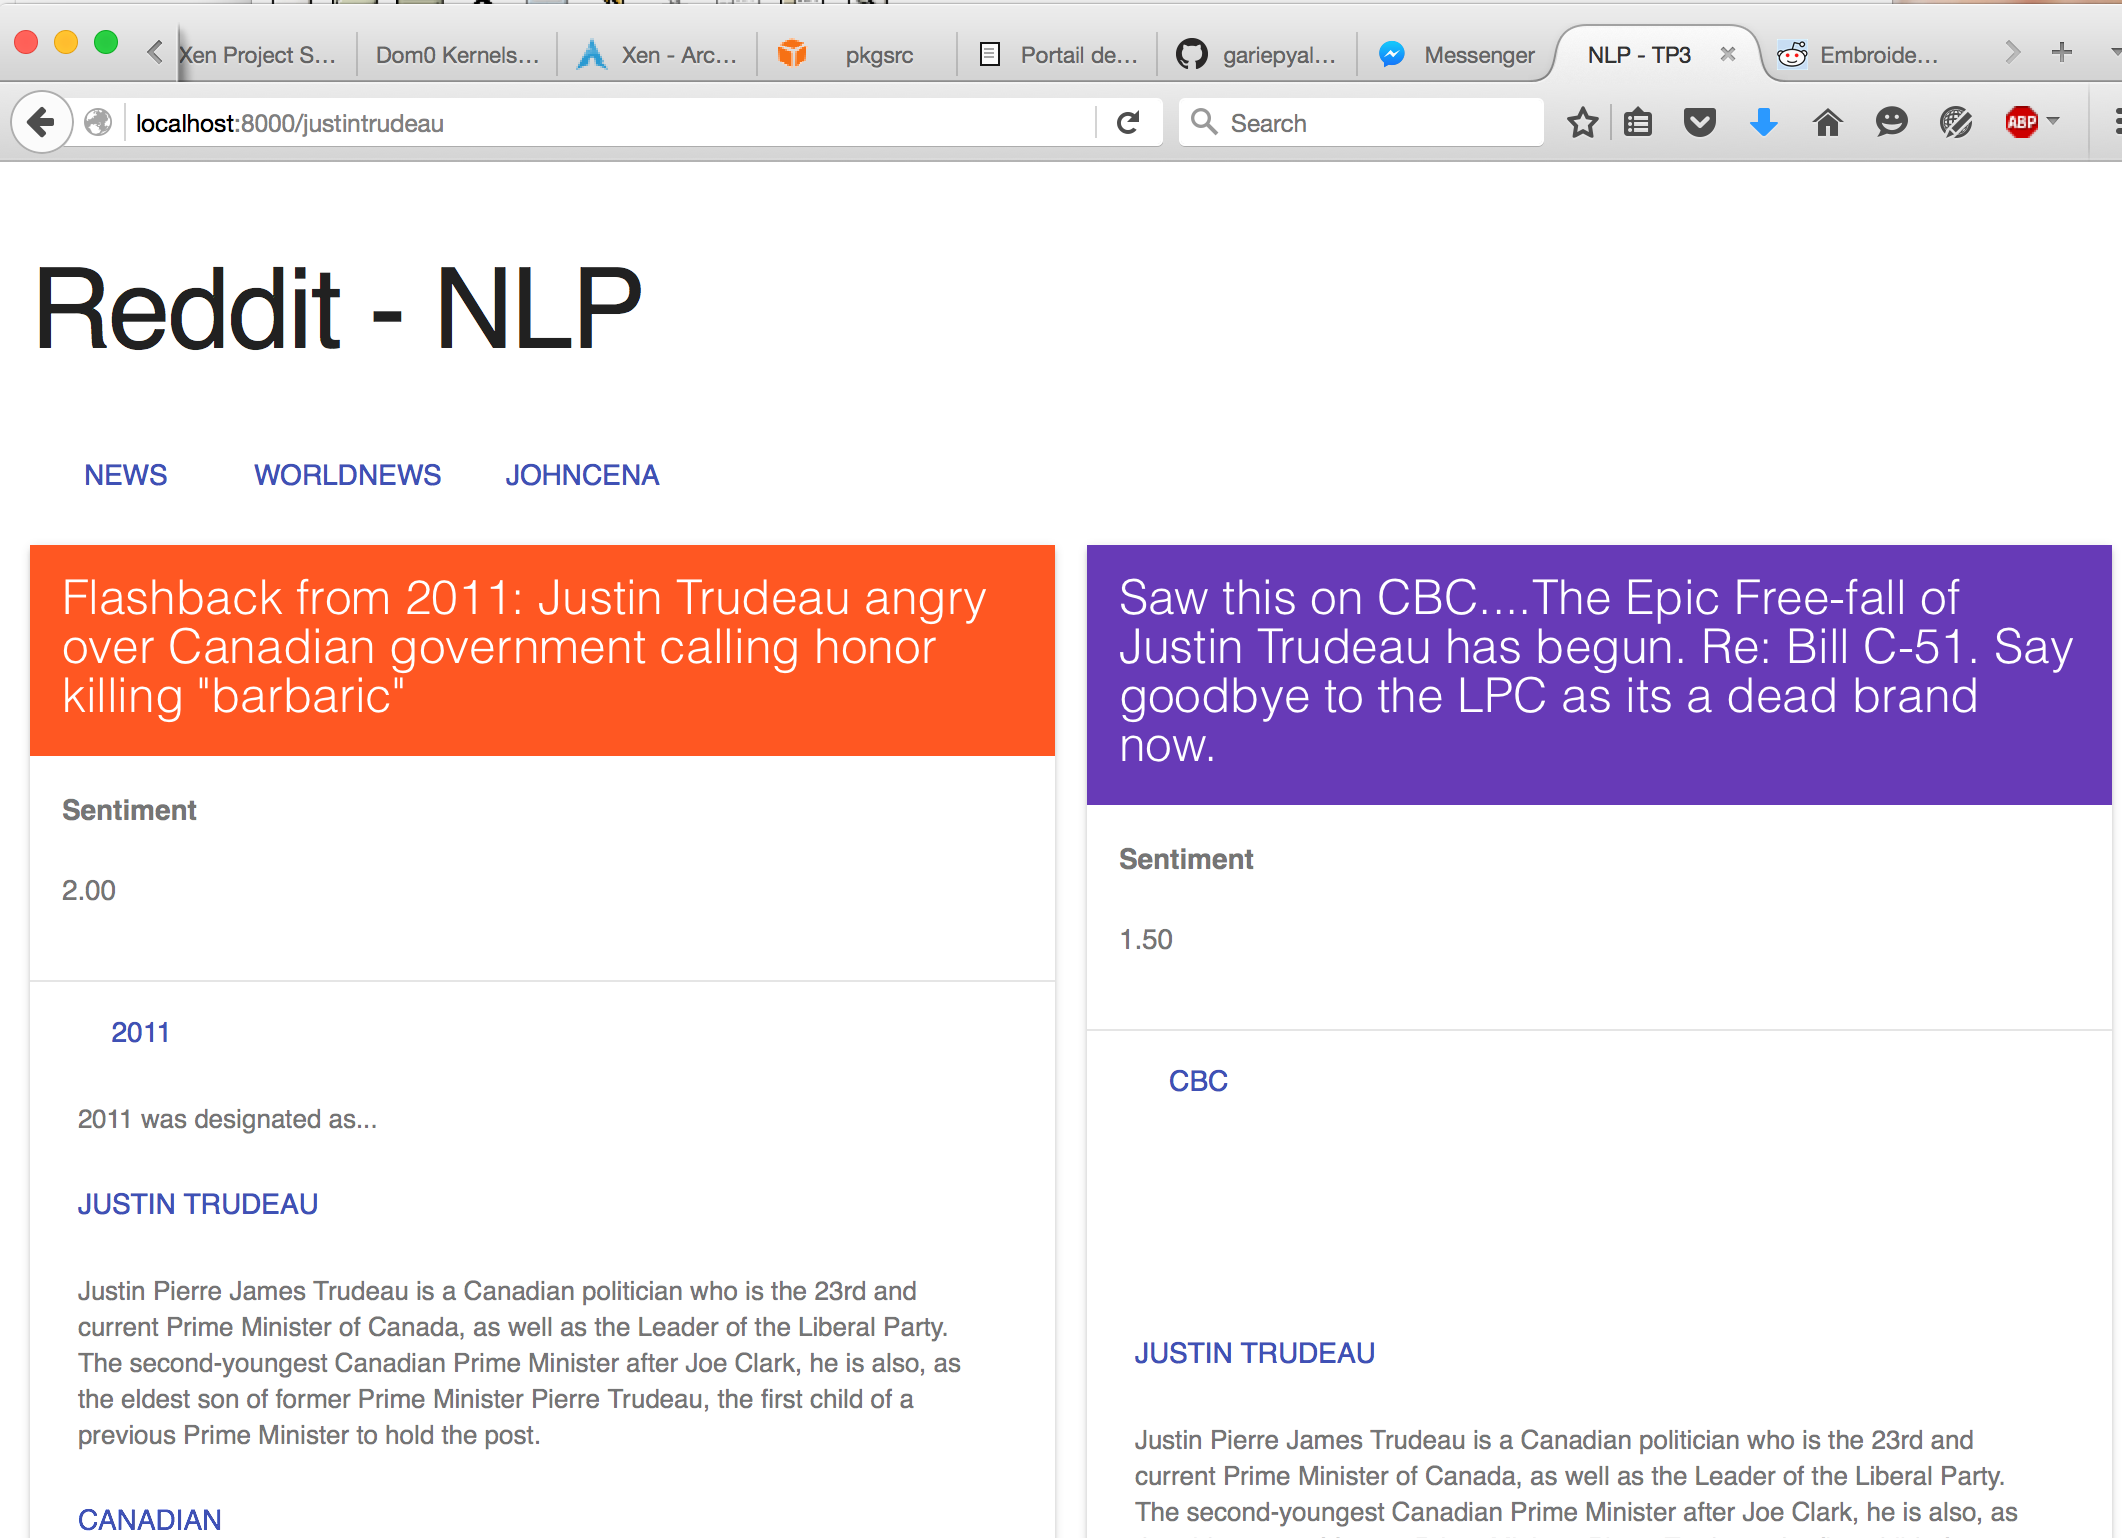
\includegraphics[width=18cm]{fig/ui-example.png}
  \label{fig:ui-example}
\end{figure}

\subsection{Synthèse des résultats}

Après l'observation de plusieurs \verb;subreddits;, on remarque une certaine tendance à la négativité des commentaires. La plupart sont sous la barre du 2, soit la neutralité. Cette tendance est possiblement attribuable au nombre de commentaires traités. Peut-être que les commentaires les plus populaires ont tendance à être les plus négatifs. Il est également possible que le jeux de données d'entraînement téléchargé ne soit pas adapté à ce genre de corpus qu'est \textit{reddit}. Pour ce qui est des entitées nommées analysées dans les titres, on en observe tout de même un nombre assez riche. Parfois certaines entitées évidentes pour nous, ne sont pas détectées et cela est peut-être aussi dû aux jeux d'entraînement. Pour ce qui est des \textit{Abstacts} retournés par \textit{DuckDuckGo}, on observe une bonne précision, mais un rappel qui laisse à désirer. Par contre, les liens retournés offrent un grand rappel et la précision est assez bonne.

%%%%%%%%%%%%%%%%%%%%%%%%%%%%%%%%%%%%%%%%%%%%

\end{document}
